% This file was created by matlab2tikz.
%
%The latest updates can be retrieved from
%  http://www.mathworks.com/matlabcentral/fileexchange/22022-matlab2tikz-matlab2tikz
%where you can also make suggestions and rate matlab2tikz.
%
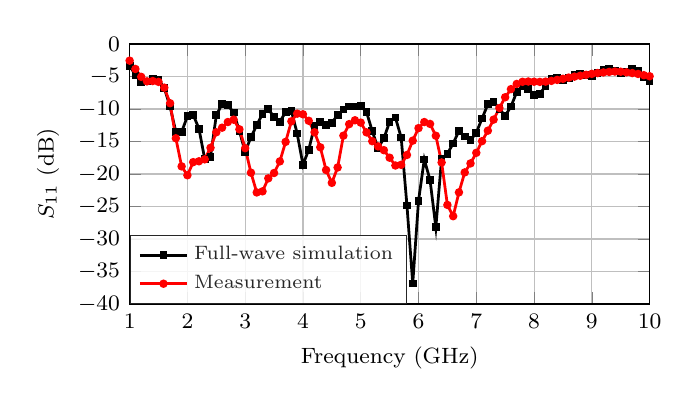
\begin{tikzpicture}

\begin{axis}[%
width=2.6in,
height=1.3in,
at={(0in,0in)},
scale only axis,
xmin=1,
xmax=10,
xminorticks=true,
xtick={1,2,3,4,5,6,7,8,9,10},
xlabel style={font=\color{white!15!black},font=\footnotesize},
xticklabel style = {font=\color{white!15!black},font=\footnotesize},
xlabel={Frequency (GHz)},
ymin=-40,
ymax=0,
ytick={-40,-35,-30,-25,-20,-15,-10,-5,0},
ylabel style={font=\color{white!15!black},font=\footnotesize},
yticklabel style = {font=\color{white!15!black},font=\footnotesize},
ylabel={$S_{11}$ (dB)},
axis background/.style={fill=white},
xmajorgrids,
xminorgrids,
ymajorgrids,
legend style={at={(0,0)}, anchor=south west, font=\scriptsize, legend cell align=left, align=left, draw=white!15!black, fill opacity=0.85}
]
\addplot [color=black, line width=1pt, mark=square*, mark options={solid, black},mark size=0.9pt]
  table[row sep=crcr]{%
  1	-3.33111	\\
1.1	-4.74998	\\
1.2	-5.84263	\\
1.3	-5.75769	\\
1.4	-5.30658	\\
1.5	-5.46642	\\
1.6	-6.77769	\\
1.7	-9.62786	\\
1.8	-13.51745	\\
1.9	-13.52507	\\
2	-11.11253	\\
2.1	-10.898	\\
2.2	-13.01995	\\
2.3	-17.70781	\\
2.4	-17.3236	\\
2.5	-10.97383	\\
2.6	-9.20712	\\
2.7	-9.40498	\\
2.8	-10.54449	\\
2.9	-13.39178	\\
3	-16.59073	\\
3.1	-14.31489	\\
3.2	-12.51261	\\
3.3	-10.71688	\\
3.4	-10.00093	\\
3.5	-11.24111	\\
3.6	-11.94404	\\
3.7	-10.4779	\\
3.8	-10.27341	\\
3.9	-13.78027	\\
4	-18.57325	\\
4.1	-16.25699	\\
4.2	-12.6412	\\
4.3	-11.97034	\\
4.4	-12.46172	\\
4.5	-12.13871	\\
4.6	-10.89088	\\
4.7	-10.08059	\\
4.8	-9.62857	\\
4.9	-9.62319	\\
5	-9.55713	\\
5.1	-10.45938	\\
5.2	-13.42594	\\
5.3	-16.02091	\\
5.4	-14.51231	\\
5.5	-11.97698	\\
5.6	-11.28869	\\
5.7	-14.38155	\\
5.8	-24.8441	\\
5.9	-36.84053	\\
6	-24.12707	\\
6.1	-17.75386	\\
6.2	-20.93869	\\
6.3	-28.20158	\\
6.4	-17.61089	\\
6.5	-16.88302	\\
6.6	-15.2859	\\
6.7	-13.37426	\\
6.8	-14.22836	\\
6.9	-14.79604	\\
7	-13.64157	\\
7.1	-11.45797	\\
7.2	-9.27046	\\
7.3	-8.86187	\\
7.4	-9.9823	\\
7.5	-11.03455	\\
7.6	-9.62183	\\
7.7	-7.38549	\\
7.8	-6.44632	\\
7.9	-6.88857	\\
8	-7.8091	\\
8.1	-7.66494	\\
8.2	-6.44477	\\
8.3	-5.40863	\\
8.4	-5.26204	\\
8.5	-5.53054	\\
8.6	-5.26936	\\
8.7	-4.72927	\\
8.8	-4.54976	\\
8.9	-4.77015	\\
9	-4.93549	\\
9.1	-4.48184	\\
9.2	-3.90615	\\
9.3	-3.79171	\\
9.4	-4.16971	\\
9.5	-4.51762	\\
9.6	-4.23164	\\
9.7	-3.89858	\\
9.8	-4.13978	\\
9.9	-5.03423	\\
10	-5.77259	\\
};
\addlegendentry{Full-wave simulation}

\addplot [color=red, line width=1pt, mark=*, mark options={solid, red},mark size=1pt]
  table[row sep=crcr]{%
  1	-2.55893	\\
  1.1	-3.83739	\\
  1.2	-5.04675	\\
  1.3	-5.73883	\\
  1.4	-5.69275	\\
  1.5	-5.82488	\\
  1.6	-6.71431	\\
  1.7	-9.10732	\\
  1.8	-14.49791	\\
  1.9	-18.8227	\\
  2	-20.18763	\\
  2.1	-18.17184	\\
  2.2	-18.03727	\\
  2.3	-17.74052	\\
  2.4	-15.96435	\\
  2.5	-13.57457	\\
  2.6	-12.87207	\\
  2.7	-11.99989	\\
  2.8	-11.63441	\\
  2.9	-13.11917	\\
  3	-16.02329	\\
  3.1	-19.79482	\\
  3.2	-22.83237	\\
  3.3	-22.66181	\\
  3.4	-20.66372	\\
  3.5	-19.83988	\\
  3.6	-18.05593	\\
  3.7	-15.05104	\\
  3.8	-11.88714	\\
  3.9	-10.7098	\\
  4	-10.81057	\\
  4.1	-11.80966	\\
  4.2	-13.57683	\\
  4.3	-15.88425	\\
  4.4	-19.3831	\\
  4.5	-21.35619	\\
  4.6	-18.9916	\\
  4.7	-14.09848	\\
  4.8	-12.32319	\\
  4.9	-11.72893	\\
  5	-12.09033	\\
  5.1	-13.59224	\\
  5.2	-14.95205	\\
  5.3	-15.74546	\\
  5.4	-16.33055	\\
  5.5	-17.49137	\\
  5.6	-18.68648	\\
  5.7	-18.57803	\\
  5.8	-17.06729	\\
  5.9	-14.86241	\\
  6	-12.93723	\\
  6.1	-12.00305	\\
  6.2	-12.29169	\\
  6.3	-14.11232	\\
  6.4	-18.21852	\\
  6.5	-24.7522	\\
  6.6	-26.48552	\\
  6.7	-22.82014	\\
  6.8	-19.75012	\\
  6.9	-18.36522	\\
  7	-16.73814	\\
  7.1	-14.93871	\\
  7.2	-13.33153	\\
  7.3	-11.62678	\\
  7.4	-9.84971	\\
  7.5	-8.18914	\\
  7.6	-6.9396	\\
  7.7	-6.14099	\\
  7.8	-5.81026	\\
  7.9	-5.76534	\\
  8	-5.8015	\\
  8.1	-5.82558	\\
  8.2	-5.78329	\\
  8.3	-5.66781	\\
  8.4	-5.52049	\\
  8.5	-5.34614	\\
  8.6	-5.16545	\\
  8.7	-5.01348	\\
  8.8	-4.87897	\\
  8.9	-4.732	\\
  9	-4.58628	\\
  9.1	-4.46445	\\
  9.2	-4.37088	\\
  9.3	-4.28759	\\
  9.4	-4.23362	\\
  9.5	-4.25958	\\
  9.6	-4.35417	\\
  9.7	-4.46681	\\
  9.8	-4.60208	\\
  9.9	-4.79543	\\
  10	-4.95766	\\
};
\addlegendentry{Measurement}
\end{axis}

\end{tikzpicture}%